\documentclass[onecolumn]{article}
\usepackage{graphicx}
\usepackage{amsmath}
\usepackage{hyperref}
\usepackage{float}
\restylefloat{figure}

\begin{document}

\title{Discontinuities and differential equations}

\author{Arjen Markus}

\maketitle

%------------------------------------------------------------------------------

\section*{Introduction}
Discontinuities in differential equations pose mathematical, analytical and numerical problems, but
they occur quite often in practice, for instance a thermostat may abruptly switch on the heating system if the
temperature gets too low or you have a point source of some contaminant in a river. In this note
a number of typical, but simple, situations are examined, where discontinuities play a role.
However, we take an engineering approach: we simply assume a solution exists and try to find it
with elementary means. Furthermore the examples all have a clear technical or environmental interpretation.

For theoretical expos\'es, see for instance:
\begin{itemize}
\item
On Discontinuous Differential Equation, Differential Inclusions and Optimal Control, \cite{OnDiscontinousDifferentialEqs}
\item
Solving ODEs and DDEs with Impulses, \cite{SolvingODEsDDEs}
\item
A Review of Recent Developments in Solving ODEs, \cite{ReviewRecentDevelopments}
\item
The Treatment of Derivative Discontinuities in Differential Equations, \cite{TreatmentDerivativeDiscontinuities}
\item
Discontinuities in ODEs, \cite{DiscontinuitiesODEs}
\end{itemize}

\section*{Switching on a source term}
The first example is very simple: we have, say, a thermostat or a stirred tank reactor and at some moment
in time we turn on the heater or we continuously input a reactant into the tank. A model equation for
this is:
%
\begin{align}
    \frac{dy}{dt} &= -y + H(t-1)
\end{align}

where $y$ is the concentration of the reactant or the temperature, the term $-y$ represents losses due to
heat exchange or chemical reactions. The function $H(x)$ is the Heaviside step function\footnote{The value for $x = 0$ is somewhat arbitrary -- see for more information \url{http://mathworld.wolfram.com/HeavisideStepFunction.html}}:
%
\begin{align}
              H(x) =
              \begin{cases}
              0 \quad \text{if} \quad x < 0     \\
\nonumber     1 \quad \text{if} \quad x \geq 0
              \end{cases}
\end{align}

As boundary condition we have:
%
\begin{align}
    y = 0 & \quad \text{at} \quad t = 0
\end{align}

\begin{figure}
\begin{center}
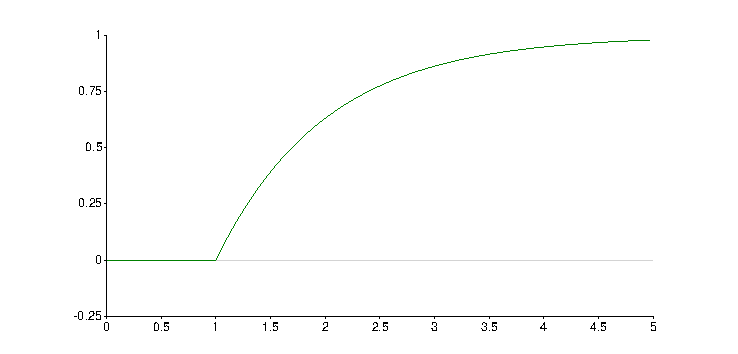
\includegraphics{jumpexact.pdf}
\caption{Exact solution for the first problem, a jump in the source term at $t = 1$.}
\label{solutionSourceOn}
\end{center}
\end{figure}

We can easily obtain the analytical solution for $t < 1$ and for $t > 1$, as the jump
discontinuity does not occur in these intervals:
%
\begin{align}
             y = &
             \begin{cases}
             A e^{-(t-1)}     & \quad \text{if} \quad t < 1 \\
             1 - B e^{-(t-1)} & \quad \text{if} \quad t > 1
             \end{cases}
\end{align}

The unknowns $A$ and $B$ can be determined by the boundary condition at $t = 0$ and by the \emph{continuity}
of the solution at $t = 1$ (see Fig.\ \ref{solutionSourceOn}).
%
\begin{align}
             A = 0 \\
\nonumber    B = 1
\end{align}

\begin{figure}
\begin{center}
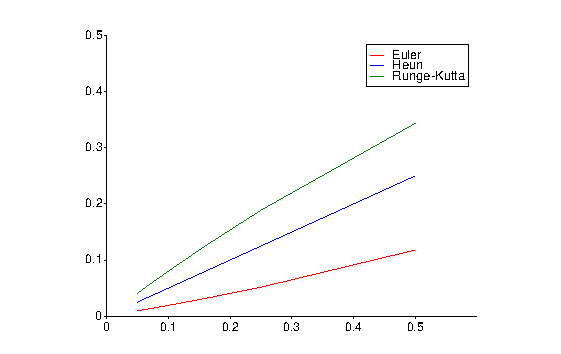
\includegraphics{jump1.pdf}
\caption{Maximum difference between the numerical solution and the exact solution as function
of the step size. The solution was obtained over the interval $[0,5]$.}
\label{figJump1}
\end{center}
\end{figure}


Now, consider what happens with well-known numerical methods, Euler, Heun and fourth-order Runge-Kutta
(see Fig.\ \ref{figJump1}). In the figure the maximum difference between the numerical solution and the
exact solution over the interval $[0,5]$ is shown as a function of the step size. The Euler method, the
simplest method, leads to errors that are four times smaller than the fourth-order Runge-Kutta method.
If the differential equation contains discontinuities, the nominally best method may not necessarily
give the best results.


\section*{Infinitely short peak}
The second example is that of a very short disturbance, a sudden burst of energy for instance. We model
this with the following equation:
%
\begin{align}
    \frac{dy}{dt} &= -y + \delta(t-1)
\end{align}
The boundary condition is the same as in the first example.

The function $\delta(x)$ is the Dirac delta function, defined by:
%
\begin{align}
    \int_{-\infty}^\infty f(x) \delta(x-a) dx = f(a)
\end{align}
\noindent for all functions $f(x)$.

Again we can solve the equation in two separate intervals, but matching them is tricky: the solution
is not continuous. The way out is observing that integration over time will -- by definition -- turn the
special character of the Dirac delta function into an ordinary term:
%
\begin{align}
            \int_{1-\varepsilon}^{1+\varepsilon} \frac{dy}{dt} dt &=  - \int_{1-\varepsilon}^{1+\varepsilon} y dt + \int_{1-\varepsilon}^{1+\varepsilon} \delta(t-1) dt \\
\nonumber         y|_{x=1+\varepsilon} - y|_{x=1-\varepsilon}     &=  - \int_{1-\varepsilon}^{1+\varepsilon} y dt + 1
\end{align}

Taking $\varepsilon \rightarrow 0$, the remaining integral approximates zero:
\begin{align}
          y_+ - y_-  &=  1
\end{align}

\begin{figure}
\begin{center}
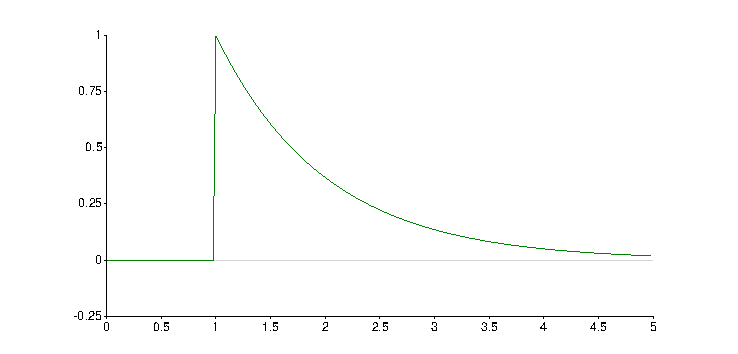
\includegraphics{jumpexact2.pdf}
\caption{Exact solution to the equation with an infinitely short peak.}
\label{solutionShort}
\end{center}
\end{figure}

In other words, there is a jump of 1 at $t = 1$. The solution is therefore (Fig. \ref{solutionShort}):
%
\begin{align}
           y =
           \begin{cases}
                 0          & \quad \text{if} \quad t < 1 \\
                 e^{(-t-1)} & \quad \text{if} \quad t > 1
           \end{cases}
\end{align}
The value at $t = 1$ is undecided, but we can take it to be 1 anyway.

The special character of the delta function makes it difficult to handle for any numerical method. It
requires specific treatment. For the Euler method this is relatively easy to do, by using the same
reasoning as above:
%
\begin{align}
            \int_{t_n}^{t_{n+1}} \frac{dy}{dt} dt &=        - \int_{t_n}^{t_{n+1}} y dt + \int_{t_n}^{t_{n+1}} \delta(t-1) dt \\
\nonumber         y_{n+1} - y_n                   &\approx
                  \begin{cases}
                  - \Delta t ~ y_n + 1  & \quad \text{if the interval} [t_n,t_{n+1}] \text{contains} t = 1 \\
                  - \Delta t ~ y_n      & \quad \text{otherwise}
                  \end{cases}
\end{align}

For a more sophisticated method like Heun's or fourth-order Runge-Kutta the reasoning goes
along the same lines.

An alternative might be to approximate the delta function via a finitely short peak of equivalent strength:
%
\begin{align}
          \Delta(x)  =
           \begin{cases}
           0             & \quad \text{if} \quad x < 0 \quad \text{or} \quad x > \varepsilon \\
           1/\varepsilon & \quad \text{otherwise}
           \end{cases}
\end{align}

In this case the solution will grow in the interval $[0,\varepsilon]$ as:
\begin{align}
     y &= \frac{1 - e^{-x}}{\varepsilon}
\end{align}

At $x = \varepsilon$, it will have grown to approximately $1 - \varepsilon/2$. So the absolute error would be
in the order of~$\varepsilon$.

\section*{Diffusion of oxygen}

\begin{figure}
\begin{center}
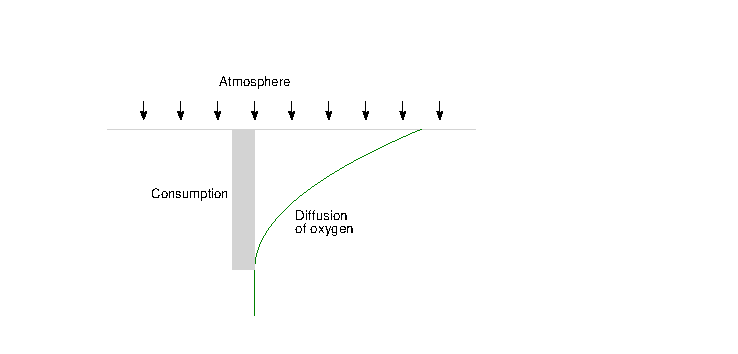
\includegraphics{diffusion.pdf}
\caption{Sketch of the diffusion of oxygen into a soil layer.}
\label{diffusionSketch}
\end{center}
\end{figure}

The next example concerns a diffusion problem, so the model equation is a second-order differential
equation. The situation is as follows (see Fig.\ \ref{diffusionSketch}): oxygen is entering a soil layer via diffusion. This gives
bacteria in the soil the opportunity to grow and thereby to consume the oxygen. We model this
process via a constant term $k$ -- unless the oxygen concentration is zero, then there is no oxygen
consumption. The model equation is:
%
\begin{align}
           D \frac{d^2C}{dz^2} - k & = 0
\end{align}
\noindent where $z$ is the vertical coordinate and $D$ is the diffusion coefficient.

The boundary conditions are:
%
\begin{align}
           C = C_0                       & \quad \text{at} \quad z = 0 \\
\nonumber  C = 0, D \frac{dC}{dz} = 0    & \quad \text{as} \quad z \rightarrow \infty
\end{align}

The problem here is that we do not know where the condition $C = 0$ will occur. If $C > 0$, as it will
be for $z$ small enough, the solution is of the form:
%
\begin{align}
\label{solutionOxygen}
           C & = A + Bz + \frac{1}{2} k z^2 / D
\end{align}
With the boundary condition $C = C_0$ at $z = 0$, we can see that $A = C_0$.

When C reaches zero, as it must, given the nature of the situation, at, say $z = \zeta$, not only
the concentration must be zero but also the flux $-D \frac{dC}{dz}$. Otherwise oxygen would be
transported into the region and that would mean the concentation would become positive and the boundary
$z = \zeta$ would shift.

Therefore, the concentration at $z =\zeta$ and the flux at $z = \zeta$ must satisfy:
%
\begin{align}
\label{eqnOxygen}
                    \left.     C \right|_\zeta = 0 &= C_0 + B \zeta + \frac{1}{2} k \zeta^2 / D \\
\nonumber  \left.  \frac{dC}{dz} \right|_\zeta = 0 &=       B       +             k \zeta / D
\end{align}

These two equations leads to:
%
\begin{align}
           B     &= - k \zeta / D \\
\nonumber  \zeta &= \sqrt{2 D C_0 / k}
\end{align}

After rearrangements we arrive at the elegant solution (see Appendix A for details):
%
\begin{align}
           C     =
           \begin{cases}
            \frac{k}{2D} (\zeta - z)^2  & \quad \text{for} \quad z \leq \zeta \\
\nonumber   0                           & \quad \text{for} \quad z \geq \zeta
           \end{cases}
\end{align}

The question is now: how to solve this problem with a numerical method? Since we have a problem with
boundaries at two sides we approach this via an evolution to an equilibrium, which allows for a simple
algorithm:
%
\begin{align}
          \frac{\partial C}{\partial t} & =
              D \frac{\partial^2 C}{\partial z^2} - k H(C)
\end{align}
The initial condition is taken as $C = 0$ and the equilibrium is reached for a large enough time $t$.

Use a straightforward discretization formula:
%
\begin{align}
          \frac{C_i^{n+1} - C_i^n}{\Delta t} & = D \frac{C_{i+1}^n + C_{i-1}^n - 2 C_i^n}{\Delta x^2} - k H(C_i)
\end{align}

We need to continue the calculation until the equilibrium profile is reached. A rough estimate for the
time span $T$, based on dimension analysis, is: $T = \zeta^2/D$. Use the following, fairly arbitrary, values
for the three parameters:
%
\begin{align}
\nonumber C_0   &= 10~g/m^3 \\
\nonumber D     &= 10^{-6}~m^2/s \\
\nonumber k     &= 10^{-3}~g/m^3 \cdot s
\end{align}
\noindent So the length and time scales are:
\begin{align}
\nonumber \zeta &= \sqrt{\frac{2DC_0}{k}} = \frac{1}{10}\sqrt{2} \approx 0.14~m \\
\nonumber T     &= \frac{\zeta^2}{D} = \frac{2}{100} \frac{1}{10^{-6}}= \approx 2 \cdot 10^4~s
\end{align}

The table below shows the results of numerical experiments with various grid cell sizes $\Delta x$.
\begin{table}[H]
\caption{Results for various grid cell sizes}
\label{tableDiffOxygen}
\begin{tabular}{lccc}
\hline
\emph{Parameter}                   & $\Delta x = 10~mm$                & $\Delta x = 3~mm$                 & $\Delta x = 1~mm$ \\
Number of cells with $C > 0$       &     $14$                          &     $47$                          &    $141$          \\
Thickness with $C > 0$             &    $0.14~m$                       &     $0.141~m$                     &    $0.141~m$      \\
Diffusion rate $- D \frac{dC}{dx}$ & $1.36 \cdot 10^{-4}~g/m^2\cdot s$ & $1.40 \cdot 10^{-4}~g/m^2\cdot s$ & $1.41 \cdot 10^{-4}~g/m^2\cdot s$ \\
\hline
\end{tabular}
\end{table}

As can be seen, the thickness of the layer with a positive oxygen concentration is quite close
to the analytical value, but the diffusion rate varies somewhat as function of the grid cell size.
This rate was calculated using the concentration in the first segment.


\section*{Continuous point source}
\label{pointSource}
Here is another situation: we have a metal beam that is heated at one point and the temperature is
kept constant at the ends. A completely different situation -- from a physical point of view -- is a channel
in which wastewater or cooling water is discharged. From a mathematical perspective both are described
with the following model equation (steady-state for simplicity):
%
\begin{align}
\label{eqnDeltaSource}
          u \frac{d T}{d x} & =
              D \frac{d^2 T}{d x^2} + h \delta(x)
\end{align}
\noindent where $h$ is the strength of the discharge, $u$ the flow velocity and $D$ the diffusion/dispersion coefficient
or the thermal conductivity.

If the flow velocity $u$ is zero, we get the beam, if it is unequal to zero, we get the river.

As the source is concentrated in a single point, the solution is simple:
%
\begin{align}
             u = 0: & \quad T = A + B x \\
\nonumber u \neq 0: & \quad T = A + B e^{u x / D}
\end{align}
\noindent where two different solutions, one for $x < 0$ and one for $x > 0$ have to be matched
(each with its own parameters).

We need suitable boundary conditions to link the two r\'egimes:
%
\begin{align}
          x = -L: & \quad T = 0  \quad \text{(suitable for both situations)} \\
\nonumber x = +L: & \quad T = 0  \quad \text{(for the beam)} \\
\nonumber x \rightarrow \infty: & \quad T ~ \text{remains~bounded}  \quad \text{(for the river)}
\end{align}

The discontinuity at $x = 0$ can be treated in a similar way as before, by integrating over a small interval
around the discharge or point of heating.

\subsection*{Heated beam}
In the case $u = 0$ (the beam), we have a solution that is
symmetric around $x = 0$. Integration over the interval $[-\varepsilon,\varepsilon]$ gives\footnote{Appendix B presents details about the units of the source term, which are not quite trivial.}:
%
\begin{align}
\label{integralDelta}
          0 & =
              D \int_{-\varepsilon}^{\varepsilon} \frac{d^2 T}{d x^2} dx + h \int_{-\varepsilon}^{\varepsilon} \delta(x) dx \\
\nonumber 0 & =
              \left. D \frac{dC}{dx}\right|_{x\downarrow 0} - \left. D \frac{dC}{dx}\right|_{x\uparrow 0} + h
\end{align}

With the symmetry condition for $T$ at $x = 0$, we can calculate $A$:
%
\begin{align}
\left. \frac{dC}{dx}\right|_{x\downarrow 0} & = - \left. \frac{dC}{dx}\right|_{x\uparrow 0} =  A \quad  \Rightarrow \quad
A = -\frac{h}{2D}
\end{align}

And with the boundary condition $T = 0$ at $x = \pm L$, we calculate $B$: $B = hL/2D$

Finally:
%
\begin{align}
          T =
          \begin{cases}
          \frac{h}{2D} (L - x) \quad \text{if} \quad x > 0 \\
\nonumber \frac{h}{2D} (L + x) \quad \text{if} \quad x < 0
          \end{cases}
\end{align}

\begin{figure}
\begin{center}
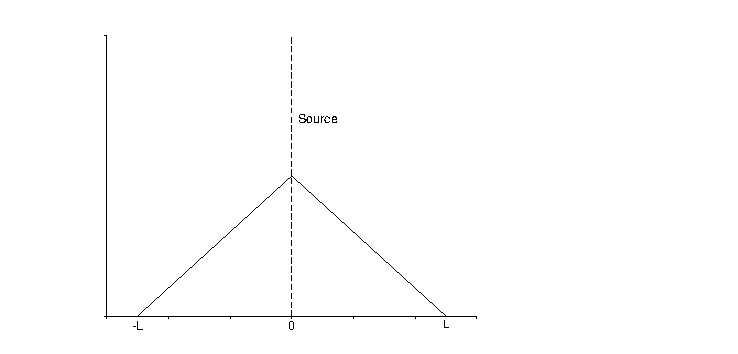
\includegraphics{bend.pdf}
\caption{Sketch of the bent solution to the "heated beam" problem.}
\label{figureBend}
\end{center}
\end{figure}

The discontinuity therefore causes a \emph{slope discontinuity} in the solution (see Fig.\ \ref{figureBend}).

One oddity of this equation is that boundaries "far away" ($L \rightarrow \infty$) cause the solution to grow indefinitely.
This is not the case in three or more dimensions nor if the flow velocity is not zero. In two
dimensions, with an axisymmetric solution, an integral over a disk surrounding the source gives,
applying Green's theorem to convert a surface integral to a contour integral:
%
\begin{align}
          0 &= D r \int_{0}^{2\pi} \frac{d T}{d r} d\phi + h \\
\nonumber 0 &= 2 \pi D r \frac{d T}{d r} + h \Rightarrow \\
\nonumber \frac{d T}{d r} &= -\frac{h}{2 \pi r D} \Rightarrow \\
\nonumber T &= A - \frac{h}{2 \pi D} \ln r
\end{align}
\noindent So the solution is not bounded for large $r$. In three dimensions, on the other hand,
with a spherically symmetric solution:
%
\begin{align}
          0 & =
              D r^2 \int_{-\pi/2}^{\pi/2} \int_{0}^{2\pi} \frac{d T}{d r} d\phi \cos \theta d\theta + h \\
\nonumber   & =
              \Bigl [D 4 \pi r^2 \frac{d T}{d x} \Bigr ]_{-\varepsilon}^{\varepsilon} + h \Rightarrow \\
\nonumber   \frac{dT}{dr} & =  -\frac{h}{4 \pi r^2 D} \Rightarrow \\
            T &=  A + \frac{h}{4 \pi r D}
\end{align}
In two and three dimensions a \emph{pole} occurs instead of a bend. The solution becomes unbounded near the
source -- there is too little surface area, you might say, but further away the influence diminishes.


\subsection*{Discharge in a river}
\label{dischargeRiver}
If there is a flow, let us assume in the positive $x$ direction (no loss of generality), then we may take
the boundaries at infinity. This actually makes the solution simpler:
%
\begin{align}
          x < 0: & \quad T = A_1 + B_1 e^{u x / D} \\
\nonumber x > 0: & \quad T = A_2 + B_2 e^{u x / D}
\end{align}
The solution must approach zero for $x \rightarrow -\infty$ and must remain bounded as $x \rightarrow +\infty$.
This immediately allows us to set $A_1 = 0$ and $B_2 = 0$. The difficulty again is the point $x = 0$ where
we need to properly match the two solutions:
%
\begin{align}
          u \int_{-\varepsilon}^{\varepsilon} \frac{d T}{d x} dx & =
              D \int_{-\varepsilon}^{\varepsilon} \frac{d^2 T}{d x^2} dx + h \int_{-\varepsilon}^{\varepsilon} \delta(x) dx \\
\nonumber u [T]_{-\varepsilon}^{\varepsilon} & =
              D [\frac{d T}{d x}]_{-\varepsilon}^{\varepsilon} + h \\
\end{align}
Filling in the above piecewise solution and taking $\varepsilon \rightarrow 0$ gives:
%
\begin{align}
          u (A_2 - B_1) & =
              D (0 - B_1 \cdot u/D) + h \\
\nonumber u A_2 & = h \Rightarrow \\
            A_2 & = h/u
\end{align}
The solution also needs to be continuous (as we have a second-order differential equation):
%
\begin{align}
          T_- = T_+ & \Rightarrow B_1 = A_2
\end{align}

\begin{figure}
\begin{center}
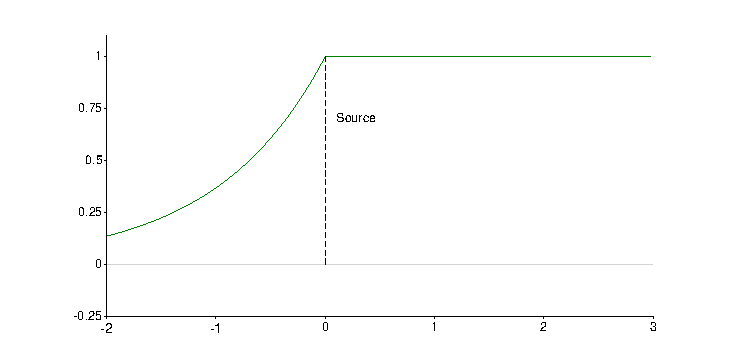
\includegraphics{river.pdf}
\caption{Typical solution to the problem of a point source in a river.}
\label{figureRiver}
\end{center}
\end{figure}

The solution is therefore (see Fig.\ \ref{figureRiver}):
%
\begin{align}
          x < 0:    & \quad T = (h/u) \  e^{u x / D} \\
\nonumber x \geq 0: & \quad T = h/u
\end{align}


\section*{A simple model of a thermostat}
Consider a straightforward model of a thermostat: the temperature in the chamber is to be kept at
some preset value $T_1$, while the outside temperature is $T_0 < T_1$. If the temperature inside the chamber
drops below $T_1$, the heating is turned on, otherwise it is off. With a heat capacity of $mc_p$
($m$ the mass of the chamber and $c_p$ the specific heat capacity), a heat exchange coefficient of $h$
and a heating rate of $q$, we can write the heat balance as:
%
\begin{align}
    m c_p \frac{dT}{dt} &= h (T_0 - T) + q H(T_1-T)
\end{align}

Applying linear scaling to the temperature and time we can simplify this to:
%
\begin{align}
    \frac{dy}{dx} &= -(1+y) + \alpha H(-y)
\end{align}

\noindent where:
%
\begin{align}
    y      &= \frac{T - T_1}{T_1 - T_0} \\
    x      &= (h/m c_p) t \\
    \alpha &= \frac{q}{h(T_1-T_0)}
\end{align}

We have three r\'egimes: $\alpha < 1$, $\alpha > 1$ and the limit case $\alpha = 1$.

First consider $\alpha < 1$:\footnote{We implicitly assume the initial temperature is below the set temperature}
the heating device is not capable of maintaining the set temperature
$T_1$ and as a consequence, the heater will be on all the time, so that $-y > 0$ and:
%
\begin{align}
    0 &= -(1 + y) + \alpha \Rightarrow y = \alpha - 1 < 0
\end{align}

In other words: the thermostat system will reach an equilibrium temperature lower than the set temperature.
The heating will be on all the time.

Secondly, consider $\alpha > 1$. If the initial temperature is below $T_1$ (y < 0), then:
%
\begin{align}
    \frac{dy}{dx} &= -(1 + y) + \alpha = \alpha - 1 - y
\end{align}

The equilibrium is therefore, if the heating was continued: $y = \alpha - 1 > 0$. The dynamical
solution is ($y(0) = y_0$):
%
\begin{align}
    y &= \alpha - 1 - (y_0 - \alpha + 1) e^{-x}
\end{align}

As soon as $y = 0$ is reached, the heating turns off and $y = 0$ should be maintained. Actually,
this is not possible within this model: if the heating is turned off, the temperature will drop below
$T_1$ and then immediately the heating is turned on again. The converse is true if the heating is turned on:
as soon as this happens, the temperature will rise above $T_1$ and therefore the heating is turned off.
There is, within this simple mathematical model, \emph{no equilibrium or even a proper solution possible}.

For a numerical method, this is an awkward situation, as "no possible solution" is not attainable. To gain
some insight, consider Euler's method:
%
\begin{align}
    y_{n+1} &= y_n + \Delta x \cdot (\alpha - 1 - y_n) \quad \text{if} \quad y_n < 0 \\
            &= y_n - \Delta x \cdot (1 + y_n)          \quad \text{if} \quad y_n > 0
\end{align}

If $y_n$ is close enough to zero, an (irregular) oscillation results - see Fig.~\ref{figThermostat}.
Similar oscillations occur when the initial temperature is above the set temperature.
The amplitude of the oscillations may be made arbitrarily small, by choosing a ever smaller time step.
But the fundamental problem continues to exist: the system is "impossible". The mathematical explanation
for this is that the Lipschitz condition is not fulfilled and therefore solutions to the corresponding
differential equation are not guaranteed to be unique or even to exist.

\begin{figure}
\begin{center}
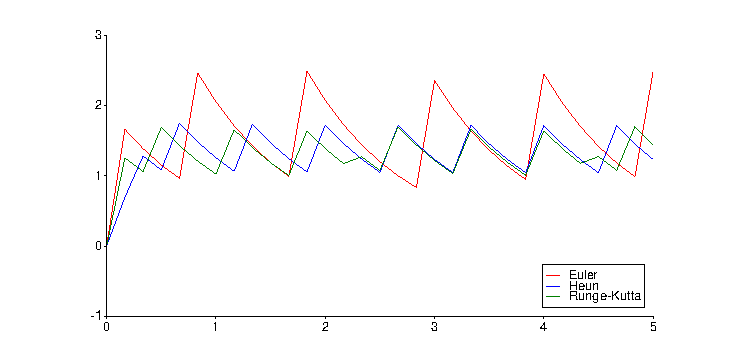
\includegraphics{thermostat.pdf}
\caption{Numerical solution for a thermostat. In this case: $\alpha = 10$.}
\label{figThermostat}
\end{center}
\end{figure}

The third r\'egime is the limit case $\alpha = 1$. This is a rather peculiar mixture of the other two:
\begin{itemize}
\item
If the initial temperature is below the set temperature, then:
%
\begin{align}
    \frac{dy}{dx} &= -(1 + y) + \alpha = -y \Rightarrow \\
                y &= y_0 e^{-x} \rightarrow 0 ~for ~x \rightarrow \infty
\end{align}

\noindent so the temperature will continue to rise up to $T_1$ ($y = 0$), but not above it.
\item
If the initial temperature is above $T_1$ ($y_0 > 0$):
%
\begin{align}
    \frac{dy}{dx} &= -(1 + y)\Rightarrow \\
\nonumber       y &= -1 + (y_0 + 1) e^{-x} \rightarrow -1 \quad \text{for} \quad x \rightarrow \infty
\end{align}
\noindent so the system will strive for an equilibrium at $T_0$ ($y = -1$). Hence it reaches the
set temperature ($y = 0$) in a finite time and then the mathematical difficulty we saw before occurs
again. For a numerical method nothing much changes: either a continuous heating an slowly rising
temperature or the odd oscillation with the heating switching on and off.
\end{itemize}

To be complete, consider the case that the initial temperature $T(0)$ is above the set temperature $T_1$ ($y(0) = y_0 > 0$).
During the first period, the heating will be off:
%
\begin{align}
    y &= (y_0 + 1) e^{-x} - 1
\end{align}

At some point in time the set temperature is reached, since the outside temperature $T_0$ is lower than $T_1$.
From this point onwards the heating will be on and we get the solution:
%
\begin{align}
    y &= (\alpha - 1) (1 - e^{-x})
\end{align}
\noindent if $\alpha < 1$. Nothing odd happens.

With $\alpha > 1$ though, the first period will be the same, a steady decrease of the temperature,
but in the second period we enter the awkward situation again that there is no analytical solution.

\section*{Cooling water discharge in a river}

\begin{figure}
\begin{center}
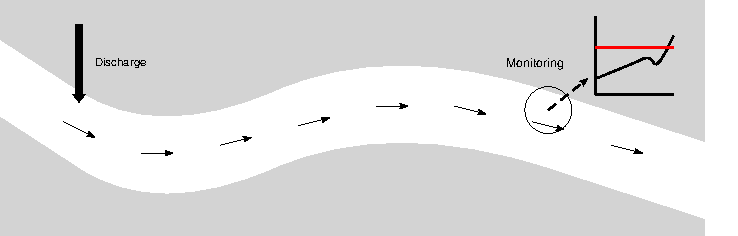
\includegraphics{river_sketch.pdf}
\caption{Sketch of a cooling water discharge in a river.}
\label{riverSketch}
\end{center}
\end{figure}

The final situation we will be investigating is that of a discharge of cooling water in a river (see Fig.\ \ref{riverSketch}). The
problem is that the temperature increase downstream may not be too large, as otherwise the environment
is harmed. If this happens, the discharge is turned off. The model equation is:
%
\begin{align}
    \frac{\partial T}{\partial t} + u \frac{\partial T}{\partial x} &= D \frac{\partial^2 T}{\partial x^2} +
                \frac{q}{\rho c_p} H(T_{max} - T(l)) \cdot \delta(x) - h(T - T_{air})
\end{align}

\noindent where in this case, the $\delta$-function is location-dependent and the Heaviside function depends
on the temperature in the monitoring point, a distance $l$ downstream from the source.

There is no actual need to solve the equation. We can sketch the behaviour based on our understanding of the physics. We need
an initial condition and two boundary conditions. The initial condition will be simply: $T = 0$ at $t = 0$.
The first boundary condition is: $T = 0$ at $x \rightarrow -\infty$. The second boundary is:
$T$ remains bounded as $x \rightarrow \infty$. In this respect it resembles the earlier case (see Section \ref{dischargeRiver}).

For the time that the temperature at $x = l$ is below the threshold, the solution is indeed similar
to that of Section \ref{dischargeRiver}. The only complication is the time-dependency: as the discharged
water is transported along the river, it will at some moment reach the monitoring point. If the temperature
is then larger than the maximum allowable temperature, the discharge is shut off. From then on the river
water will have the ambient temperature. When that water reaches the monitoring point, the temperature
no longer violates the standard and the discharge can be turned on ... leading to a cyclic behaviour
(see Fig.\ \ref{cyclicBehaviour}).

\begin{figure}
\begin{center}
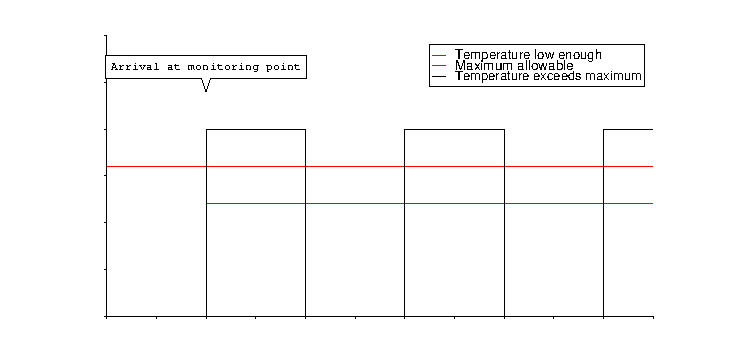
\includegraphics{cyclic.pdf}
\caption{Sketch of the water temperature in the monitoring point.}
\label{cyclicBehaviour}
\end{center}
\end{figure}

Since there is no alternative for the cooling water discharge, it is either on or off, the system
cannot reach an equilibrium, if the temperature will exceed the maximum allowable temperature. This is
a direct consequence of the discontinuity.


%------------------------------------------------------------------------------

\subsection*{Appendix A: Details of the derivation of the solution in "Diffusion of oxygen"}
\label{appOxygen}
The second part of equations \ref{eqnOxygen} directly leads to:
%
\begin{align}
         B &= -k\zeta/D
\end{align}

Substitution into the first part gives:
%
\begin{align}
         0 &= C_0 -k\zeta^2/D + \frac{1}{2} k\zeta^2/D
\end{align}
\noindent and therefore:
%
\begin{align}
         0 &= C_0 - \frac{1}{2} k\zeta^2/D \Rightarrow \zeta = \sqrt{2DC_0/k}
\end{align}

When we substitute these expressions into equation \ref{solutionOxygen}, we get:
\begin{align}
          C &= C_0 - k\zeta z / D + \frac{1}{2} k z^2/D \\
\nonumber   &= \frac{1}{2} k \zeta^2 / D - k\zeta z / D + \frac{1}{2} k z^2 / D \\
\nonumber   &= \frac{k}{2D} (\zeta^2 - 2 \zeta^2 z + z^2) \\
\nonumber   &= \frac{k}{2D} (\zeta - z)^2)
\end{align}


\subsection*{Appendix B: Units in section on Continuous point source}
\label{appUnits}
The problem presented in Section \ref{pointSource} has an aspect peculiar to the physical interpretation:
the units in which the various terms are to be expressed. Equation \ref{eqnDeltaSource} has terms with a
unit $[m/s \cdot K/m] = [K/s]$. This is straightforward, but it means that the term $h\delta(x)$ also
has this unit. When we integrate over a short interval $[-\varepsilon,\varepsilon]$ (equation \ref{integralDelta})
it becomes clear that the strength of the heating $h$ must have a unit $[Km/s]$.

This can only be the case, because the $\delta$ function has a unit $[m^{-1}]$ -- something that is never
an issue when you look at it from a pure mathematical viewpoint.

But how to interpret this unit? Consider the beam (or the river): the one-dimensional equation actually
refers to a three-dimensional beam in which the temperature is uniform over the cross-section. So the
source, be it heat or a pollutant, actually has a unit $[Km^3/s]$ and obtains, \emph{as a sectionally
averaged quantity}, the unit $[Km/s]$.

\bibliography{discontinuities}
\bibliographystyle{unsrt}
\end{document}
